\chapter{Introduction}
\label{chapter:intro}
In the study of cosmology -- the branch of physics dedicated to understanding how the Universe came to be and what that Universe looks like today -- galaxies are perhaps one of the most important observational tracers with which we can map and measure the structure of our Universe throughout cosmic time. As a result, robust models for the formation and evolution of galaxies are an essential aspect of the framework by which we might build a good understanding of our Universe. These collections of gas, stars and ambiguous dark matter are the direct result of the complex interplay between gravitation and electromagnetic interactions that define the Universe which we live in, and so their characteristics are immutably tied to the very nature of our existence.

Of all the galaxies in our Universe, the one to which we have the closest access to understand the nuanced aspects of its formation and evolution is the galaxy within which we reside: the Milky Way -- \emph{the} Galaxy. The Milky Way presents the problem of galaxy formation at high fidelity, allowing us to test models for its genesis and evolution on a star-by-star basis. The assumption that our Galaxy is typical for its mass and other characteristics then allows us to extrapolate these models, trained on the Milky Way, to our understanding of galaxy evolution in general. The overarching goal of this thesis is to test that assumption, by both refining our current understanding of the formation and evolution of the Galaxy, and eventually asking the question: \emph{is the Milky Way typical?}

By asking this question, we gain a means of properly calibrating any extrapolation of galaxy formation models, and will likely elucidate new aspects of the formation and history of the Milky Way through answering it. If the Milky Way \emph{is} a typical spiral galaxy, whose history is representative of the majority of galaxies at its mass and morphology, then it is a robust frame on which to develop models. If, however, the Milky Way is somehow \emph{atypical}, for example in its size, assembly history, stellar population and dark matter content or any other characteristic --  or combination of the above -- then it is important that the use of our detailed knowledge of the Milky Way should be tempered somehow to allow for these `atypicalities'. Of course, a detailed knowledge of the Milky Way only strengthens our understanding of its individual history of formation and assembly.

The means to answer this overarching question of the typicality of the Galaxy can only be established through a detailed and robust understanding of the place of our Galaxy in the Universe and its galaxy population. In this thesis I intend to make progress towards such an understanding by:
\begin{itemize}
    \item Developing a detailed and state-of-the-art picture of the present day spatial structure of the Milky Way, to act as a stringent constraint on present and future models for its formation.
    \item Understanding how galaxies with similar characteristics to the Milky Way emerged, and how these galaxies compare to the mean galaxy population, through analysis of cosmological numerical simulations that accurately reproduce the broad properties of the galaxy population.
    \item Testing the predictions of these numerical simulations by reconstructing aspects of the assembly history of the Galaxy, using the most up-to-date data on the Milky Way.
\end{itemize}
The achievement of these more concentrated goals will allow for a robust assessment of the typicality of the Galaxy, and will inform the future interpretation of models for the formation and evolution of the Milky Way in the context of external galaxies.

The remainder of this chapter is divided into three parts. The goal here is to introduce on a broad level the state-of-the-art of our understanding of the Milky Way and its formation and evolution and how this is used to understand galaxy formation on a general basis. The first section, Section \ref{sec:cosmocontext} briefly introduces galaxy formation theory from a extra-galactic viewpoint. I then present the current understanding of the present day structure and components of the Milky Way in Section \ref{sec:mwadg}. Section \ref{sec:galacticarchaeology} then broaches the middle ground between these extra-galactic and Galactic approaches, presenting the leading models for the formation of the Milky Way through cosmic time.

\section{Galaxies in the cosmological context}
\label{sec:cosmocontext}
Before considering the state of our knowledge of the formation and evolution of the Milky Way, it is essential to set the scene of our current understanding of galaxies in general, and how this may be connected -- in part -- to the structure of the Universe. To this end, I briefly touch upon here some important aspects of galaxy formation theory in the cosmological context, with the aim of placing studies of the Milky Way into their much wider setting.

\subsection{Galactic genesis}

In the current popular interpretation of modern cosmology, the cold dark matter model \citep[CDM, e.g.][]{1978MNRAS.183..341W}, galaxies are the eventual products of small scale fluctuations in the density field of the very early Universe, imprinted upon it by a rapid period of inflation very shortly after the Big Bang \citep{guth1981inflationary}. These `seed' fluctuations then collapsed under their own gravity as they became significant over the background density, which decreased with the expansion of the Universe. Dark matter, thought to interact with baryonic matter only through gravitation, filled these overdensities first, as it was not supported by the radiation which bakes the early Universe. As the density fluctuations grew with infalling dark matter, the baryonic matter slowly began to cool and collapse into the overdensities, forming the filamentary structure referred to as the `cosmic web'. The gas eventually collapsed deep into the potential wells of the dark matter, forming galaxies of great morphological variety - one of which became \emph{the} Galaxy: the Milky Way.

This simplified picture of structure formation followed by the genesis of galaxies provides a first hint at how the galaxy population of the Universe is perhaps the (indirect) result of cosmology, in that the structure of the early Universe eventually results in the galaxy population and the Galaxy. Na\"ively then, if galaxies are the `end product' of the evolution of the Universe, one might expect to `reverse engineer' the galaxy population, and say something about the nature of our Universe. In some sense, this is the one of the goals of the study of galaxy formation and evolution. However, this ideal is somewhat complicated by the non-linearity of the processes on galactic scales. This collapse and subsequent hierarchical build up of haloes following the growth of the initial density fluctuations can only be properly realised through direct numerical simulation \citep[e.g.][]{2005Natur.435..629S}. In the course of this thesis I will exploit the fact that numerical simulations, which describe the above processes self-consistently, and also accurately model the hydro-dynamical processes that shape galaxies, are currently the most robust means of predicting the context of our Galaxy within CDM and other models.

\subsection{The galaxy-halo connection}
\label{sec:galaxyhaloconnect}
The study of the observable galaxy population has a long history. The early work of \citet{1926ApJ....64..321H}, culminated in the widely known Hubble `Tuning-fork' diagram \citep[e.g.][]{1936rene.book.....H,1961hag..book.....S}. This diagram represents a useful summary of galaxy morphologies, but since that time it has become clear that the physical properties of galaxies are complicated far beyond their overall structure, and large scale surveys have revealed that they host a wide range of structures which may offer insight into their evolutionary histories \citep[e.g.][]{2009ARA&A..47..159B}. Galactic astrophysics attempts to eke out the physics behind these properties and their connection to galaxy evolution theory and thus to cosmology and constraints on the currently accepted cosmological models. 

While direct constraints on the physical origins of all the features of the galaxy population are clearly out of easy reach, `broad-brush' approaches, such as correlating certain properties of galaxies with one another, lend some insight into the problem of galaxy evolution. For example, it is well established that galaxy morphologies correlate with their colours \citep[e.g.][]{2001AJ....122.1861S}, where blue (likely star-forming) galaxies tend to be those dominated by spiral and disc structures, and red (and therefore mostly non-star forming) galaxies are generally spheroidal in morphology. However there are departures from this rule and studies such as the Galaxy Zoo project \citep{2008MNRAS.389.1179L,2011MNRAS.410..166L}, which allowed for robust, citizen science-driven, visual classification of an unprecedented sample of galaxies has shown that there are notable exceptions to this general trend \citep[e.g.][]{2009MNRAS.396..818S,2010MNRAS.405..783M}. Furthermore, galaxy colours are roughly bimodal \citep[e.g.][]{2004ApJ...600..681B,2006MNRAS.373..469B} meaning that galaxies mainly fall into either of the red or blue groups, and very few reside in the intermediate `green' valley. Such a colour bimodality suggests that if transitions between these groups occur, they occur very quickly. \citet{2006MNRAS.373..469B} showed that the fraction of galaxies in each group changes as a function of the number of a galaxy's projected neighbours, suggesting environment somehow plays a role in quenching star formation in the red, dead galaxies. \citet{2010ApJ...721..193P} separated the effects of environment and galaxy mass, demonstrating that star formation quenching is driven by both of these factors separately at different rates, where the environment tends to drive quenching mainly in satellite galaxies, and appeared to be independent of the mass of the haloes in which they reside \citep{2012ApJ...757....4P}. \citet{2013MNRAS.428.3306W} demonstrated that distance from the cluster center is a clearer defining factor of satellite quenching, and were able to reconcile the data with a dependence on halo mass. Quenching which is dependent on halo mass can be neatly framed as resulting from virial shock heating in the most massive haloes, which shuts down accretion by bringing gas cooling timescales above the dynamical time of the haloes \citep[e.g.][]{2006MNRAS.368....2D,2015MNRAS.447..374G}. Therefore, it may be that through the connection between their halo mass and colour, the galaxies as they appear to us are in some way a product of cosmology, via its dictation of the formation of structure. These results build up to a useful statement on the driving forces behind galaxy evolution, but are only one component of a comprehensive picture of the physics that forms galaxies in the variety we see.

A good example of an agent of galaxy evolution that is seemingly not \emph{directly} driven by the formation of structure (and therefore cosmology), but is extremely important in reproducing the smaller scale ($\lesssim 0.01$ Mpc) structure in the Universe, is the effect of feedback. Feedback in galaxy formation refers to the regulation of star formation, usually via the attenuation of gas inflow by some process. Generally, feedback is divided into that from stellar sources, such as energy input from supernovae (SNe) or stellar winds, or that from black holes in the central regions of galaxies, e.g. active galactic nuclei (AGN). Allowing gas to collapse into galaxies without feedback means star formation proceeds at rates far higher than that observed, leading to galaxies with stellar masses tens of times greater than those seen today. However, the inclusion of even relatively simple models for stellar feedback in early simulations and semi-analytic models brings galaxy total masses closer inline with observations at the low mass end  \citep[$M_{200}\lesssim 10^{12}\ \mathrm{M_\odot}$ e.g.][]{1996ApJS..105...19K,1999MNRAS.310.1087S,2003MNRAS.339..312S}, whereas AGN feedback is necessary to suppress star formation in more massive galaxies \citep[$M_{200}\gtrsim 10^{12}\ \mathrm{M_\odot}$][]{2006MNRAS.370..645B,2008MNRAS.391..481S}, where energy injection from SNe is insufficient to pause cold inflows or halt cooling flows from the hot coronae of galaxies. As a result of these feedback processes on both ends of the halo mass scale, the efficiency of star formation peaks in haloes with total mass $\sim 10^{12}\ \mathrm{M_\odot}$ \citep[e.g.][]{2013ApJ...770...57B} which, as I will discuss later, is roughly the halo mass of the Milky Way. 

Not only is feedback thought to be important for the regulation of galaxy stellar masses, but likely also plays some role in determining galaxy morphologies, in particular that of disc galaxies. Without sufficient feedback, low angular momentum material is not removed from central regions of simulated galaxies, which then do not reproduce properties of observed discs \citep[e.g.][and references therein]{2010MNRAS.408..812S}. However, including models for feedback that can efficiently eject such material to be re-accreted at later times with a higher angular momentum produces far more realistic discs, simulated self consistently in a cosmological context \citep[e.g.][]{2011MNRAS.415.1051B,2012MNRAS.427..379M,2013MNRAS.428..129S}. Therefore, the disc morphology of galaxies like the Milky Way is likely folded directly in with its history of feedback. Of course, stellar feedback is a direct result of the star formation history in any galaxy, which is dictated by the supply of gas at a given time. If, as I touched on above, the gas supply to haloes hosting galaxies is dictated by their mass (to first order), then this suggests that the large scale structure of the Universe, which dictates the mass function of galaxies, then also dictates the morphology distribution of galaxies. It is clear then that understanding the formation and assembly of disc galaxies in detail is an important component of galaxy evolution theory, and may help to provide insights even on cosmological scales.

Further to the above processes, which are all somewhat intrinsic to the host haloes, another important `external' process which has important effects on the evolution of galaxies is that of merging. The assembly of massive galaxies from the accretion of smaller pieces, alongside smooth accretion of gas, as discussed above, is a key prediction of the cold dark matter model \citep[e.g.][]{1974ApJ...187..425P}. The assembly of galaxies is commonly quantified by the formation time, by redshift $z_{1/2}$, which describes the redshift at which half the mass of the host halo is assembled. This time is found to be strongly related to the large scale clustering of haloes \citep[commonly referred to as assembly bias, e.g.][]{2005MNRAS.363L..66G,2007MNRAS.377L...5G}. The link between the assembly histories of galaxies and features such as their star formation history is commonly made using abundance matching models, which link the observational luminosity functions of galaxies at different redshifts to the haloes of dark-matter-only simulations. Using such a technique, \citet{2013MNRAS.428.3121M} found that haloes similar to the Milky Way assemble more than half their central stellar mass after $z=0.7$. The relationship between star formation history, stellar mass growth and dark matter assembly was studied in the EAGLE simulations by \citet{2018arXiv180505956M}, who showed that the specific star formation rate of galaxies at $z=0.1$ is strongly related to their past assembly history, which, by the link between $z_{1/2}$ and large scale structure, further suggests a connection between the formation time and the characteristics of central galaxies. In Chapter \ref{chapter:eagle}, I build on this by presenting evidence that the assembly history of the Milky Way may have an indirect connection to its light element abundances, making an argument that the Milky Way appears unusual in this respect.


\section{The Milky Way as a disc galaxy}
\label{sec:mwadg}
% Having established the place of disc galaxies in our efforts to understand the Universe, and the importance of a detailed understanding of their formation and evolution, I now move to focus solely on that aspect of galactic astrophysics. I will summarise the current understanding of the Milky Way as a disc galaxy, before briefly describing the established model of galactic disc formation. In particular, I aim to introduce the extensive literature on the Milky Way from the last century, and explore the origin and development of near-field cosmology and Galactic archaeology -- the study of the Milky Way as a fossil remnant of the process of galactic formation and evolution (perhaps more accurately expressed as Galactic paleontology!).

%Having established the importance of understanding the formation and evolution of disc galaxies in our efforts to understand the Universe, I now move to focus solely on this aspect of galactic astrophysics. Before discussing the progress thus far in understanding the history of formation and evolution of the Milky Way and other disc galaxies, I will first summarise what we know about the Milky Way as a galaxy. 

In this Section I summarise current knowledge of the main properties of the components of the Milky Way, as well as the present understanding of its history of formation and evolution. That we reside in a disc of stars was first postulated by the philosopher Immanuel Kant in 1755, shortly before William Herschel first mapped the shape of the Milky Way through star counting in 1785 \citep{Herschel01011785}. The fact that our Galaxy is just one of the many galaxies in the Universe was not properly understood until the early 20\textsuperscript{th} century, with the work of \citet{1929ApJ....69..103H}. Since that early work, we have come to be able to properly characterise our Galaxy and compare it to the others we observe, although as I will discuss, much of this knowledge is now being tested when confronted with the latest data.

Morphology and structural parameters are perhaps the most obvious features one would focus on when comparing the Milky Way with its extragalactic counterparts. Such properties are readily measured for external galaxies and have been for some time \citep[e.g.][]{1959HDP....53..311D}. In terms of morphology, it is well established that the Milky Way has an extended stellar disc with spiral arms, a bulge component, a bar and a diffuse stellar halo with evidence of substructure. The exact details of many of these features are difficult to discern owing to the fact that a substantial fraction of the Galaxy is obscured by extinction as a result of our position in the disc, but much progress has been made in the latter half of the 20th century. Here, I will give an overview of our current understanding of the structure and morphology of the Milky Way and its components. I will also discuss the connections between morphological components and trends in element abundances, with a view to later bringing these connections to bear on models for the formation of the Galaxy.

\subsection{The disc}

The disc is the component of the Galaxy which we have arguably the best hope of understanding given the ease of access to its stars, at least in the Solar vicinity. The disc forms the main focus of this thesis, as it is the one of the main components (alongside the stellar halo) for which data are readily available from large Galactic surveys. Therefore, I discuss the disc at a greater level of detail than the other components. The Galactic disc corresponds to $\sim85\%$ of the Milky Way stellar mass \citep[e.g.][]{2013A&ARv..21...61R} and has been and still is the target of many surveys of Galactic stellar populations (e.g. RAVE: \citeauthor{2006AJ....132.1645S} \citeyear{2006AJ....132.1645S}; \emph{Gaia}-ESO: \citeauthor{2012Msngr.147...25G} \citeyear{2012Msngr.147...25G}; GALAH: \citeauthor{2016arXiv160902822M} \citeyear{2016arXiv160902822M}; APOGEE: \citeauthor{2015arXiv150905420M} \citeyear{2015arXiv150905420M}).  Yet, there are still basic features of the structure and stellar population content of the disc that are not well understood.

\subsubsection{Spiral Structure}
Spiral structures are ubiquitous in stellar discs, thus providing an excellent basis for statistically robust comparisons with the Milky Way. However, our knowledge of the spiral structure is rather contentious. Mapping of the spiral structure is commonly performed in the near infra-red (NIR) and radio regime, overcoming much of the extinction to look at star forming regions of the Galaxy, where the spiral structure is thought to be most apparent. Early studies of HII regions defined the `standard model' for the spiral structure of our Galaxy as a four armed spiral close to an Sc type with a $12^{\circ}$ pitch angle  \citep{1976A&A....49...57G}. However, at the turn of the century, studies of Galactic spiral structure were struggling to agree on the number of arms between two and four \citep[e.g.][]{1976A&A....46..261S,1980ApJ...239L..53C,1981ApJ...250..551B,1995ApJ...454..119V,2000A&A...358L..13D,2003A&A...397..133R}, generally because of the difficulties in measuring distances. However, Very Long Baseline Interferometry (VLBI) meaurements, which allow direct and precise trigonometric parallax and proper motion measurements favour a four armed spiral structure \citep{2009ApJ...700..137R,2014ApJ...783..130R}, and more recent measurements of young stellar populations also confirm this picture \citep{2014MNRAS.437.1791U,2015MNRAS.450.4150C}. It seems that much of this contention arises in the age of the tracer used, with those tracing older populations in the NIR \citep[e.g.][]{2000A&A...358L..13D} favouring two armed models. This suggests that the Galaxy may in fact appear to an external observer as some superposition of two and four armed. 

The physical nature of the spiral arms is also the subject of much debate, splitting into two main streams between long lived stationary density wave models \citep[e.g.][]{1964ApJ...140..646L,1996ssgd.book.....B}, and models where the arms are transient and recurrent through the history of the disc \citep[e.g.][]{1981seng.proc..111T,1984ApJ...282...61S}. It is well established that tidal forces from satellites can give rise to transient spirals \citep[e.g.][]{2010MNRAS.403..625D}, but spiral patterns do still arise in isolated simulations of thin discs. Indeed, the lifetime of the spiral arms appears to be one of the more important questions to ask, which would discrimate between these models \citep{2011MNRAS.410.1637S}. In a recent example of how such a discrimination might be made, \citet{2018MNRAS.481.3794H} modelled the velocity field in the solar neighbourhood under the effects of transient winding spiral arm perturbations and found good agreement with \emph{Gaia} DR2 data. 

\subsubsection{Size and Thickness}
\label{sec:discsize}
The vertical extent of the disc is relatively well characterised at the solar radius due to the relative lack of extinction at high Galactic latititudes. For a long time, the disc has been divided into a thick and thin component, owing to the early results of \citet{1983MNRAS.202.1025G}, and the knowledge that such structures appear to exist in external disc galaxies \citep[e.g.][]{1979ApJ...234..829B,1979ApJ...234..842T,2006AJ....131..226Y}. Of many different measurements, a good baseline for the characteristic heights of these disc components is found in the tomography of M dwarfs from SDSS data in \citet{2008ApJ...673..864J}, who find exponential scale heights of 300 and 900 pc for the thin and thick component, respectively. In this sense, the Milky Way sits relatively well with external galaxy measurements, which have similar scale heights and also have radially extended thick components \citep[e.g][]{2006AJ....131..226Y}. However, the simplified view of these components as separate geometric entities breaks down somewhat when the disc is dissected further.

A more natural separation can be made in the disc in its $\alpha$ element abundances (which is discussed further in Section \ref{sec:discabundances}), whereby the disc can be divided into a high and low-\afe{} component \citep[e.g.][]{1998A&A...338..161F,2003A&A...410..527B,2005A&A...433..185B,2013A&A...560A.109H,2014A&A...562A..71B,2014A&A...564A.115A,2014ApJ...796...38N,2015ApJ...808..132H}. These components are found to have similarities to the geometrically divided thin/thick disc, such that the high-\afe{} disc has scale height $\sim 1$ kpc, and the low-\afe{} disc has a scale height as low as $\sim 0.2$ kpc \citep[e.g.][]{2012ApJ...753..148B,2016ApJ...823...30B}. However, when defined in this way, the high-\afe{} component has a relatively short scale length at $\sim 2$ kpc, compared to the geometrically defined thick disc which has a scale length closer to $\sim4$ kpc \citep{2008ApJ...673..864J}. The low-\afe{} component has a flatter radial profile \citep{2012ApJ...752...51C}, which has a complex density structure resembling donut-shaped annuli, such that the density increases out to a break radius, and decreases outside this radius \citep{2012ApJ...753..148B,2016ApJ...823...30B}. Furthermore, when the disc is divided into sub-populations according to the \afe{} and \feh{}\footnote{Throughout, element abundances [X/Y] are defined as the base 10 logarithm of the ratio of the abundance of the elements X and Y, relative to the ratio of these elements in the Sun i.e. $\mathrm{[x/y]} = \log_{10}(\mathrm{X^{x}/X^{y}})-\log_{10}(\mathrm{X^{x}_{\odot}/X^{y}_{\odot}})$, where $X^{x}$ denotes the abundance (by number or mass) of the element x (for clarity, this definition is fully expressed also in Chapter \ref{chapter:eagle})} abundances of its stars, it seems that the vertical mass distribution is smooth, suggesting that the `thick' disc may not be so distinct \citep{2012ApJ...751..131B}. Combining all the sub-populations, this can be reconciled with the double exponential found in the star counts by \citet{1983MNRAS.202.1025G} \citep[see][]{2013A&ARv..21...61R}. The vertical kinematics of the disc as a function of \afe{} are consistent with a smooth vertical structure \citep{2012ApJ...755..115B}, and it is clear that the high-\afe{} disc is more kinematically hot than the low-\afe{} stars \citep[e.g.][]{2005A&A...433..185B}. It is clear, therefore, that the link between the disc structure and its element abundances may be able to offer significant insight into the formation and evolution of the Galaxy. In Chapter \ref{chapter:apogeestruc}, I specifically study the structure of the disc not only as a function of \afe{} and \feh{}, but also in stellar age, attempting to further understand the origin of these disc components.

Regardless of how the disc is divided and measured, it seems that when all populations are combined the Milky Way is characterised by a disc scale length in the region of $\sim 3$ to $4$ kpc \citep{2008ApJ...673..864J}. However, without an unbiased estimate of the mass in the high and low-\afe{} discs it is difficult to place a single value on this parameter based on the density modelling procedures described above. Dynamical measurements place even smaller estimates on this parameter, at roughly $2$ kpc \citep{2013ApJ...779..115B}. External disc galaxies with similar stellar mass to the Milky Way seem to have much larger discs, with mean scale lengths closer to $\sim 4$ kpc \citep[e.g.][]{2010MNRAS.406.1595F} and our nearest massive disc, the Andromeda galaxy (M31), has a large scale length in the region of $5$ kpc \citep[e.g.][]{2011ApJ...739...20C}. Therefore, it appears that the Milky Way is certainly \emph{atypical} in this regard. This is, in fact, one of the most notable characteristics that we know to set the Milky Way aside from its disc galaxy counterparts. It remains to be seen whether this is simply an effect of the different measurement methods required to measure this feature in external galaxies and the Milky Way.

\subsubsection{Element Abundances}
\label{sec:discabundances}
Disentangling the origins of element abundance patterns in the solar vicinity and beyond offers many constraints on models for the formation of the Galaxy and its star formation history \citep[seminal reviews on the goals of this effort are given by][]{1997ARA&A..35..503M,2002ARA&A..40..487F}. A good first order tracer of the history of star formation in the Galactic disc is offered by the metallicity of stars, as measured by their \feh{} abundance. Iron, as the primary ejecta of Type Ia supernovae (SNe), is a good indicator of the advancement of star formation in stellar populations. However, as I will discuss, the ratio of Iron abundance to that of the $\alpha$-elements, \afe{}, is a potentially more constraining diagnostic of the history of star formation in the disc. The many other element abundances which can be measured that originate from various sources are of course of great importance in understanding the history of the Milky Way, but I do not focus on these here.

Most models try to predict metallicity gradients in the disc and how these evolve over time. Metallicity gradients are measured by a variety of tracers by which the variation in the gradient with age can also be measured, including planetary nebulae \citep[e.g.][]{1994A&A...282..436M,1994Ap&SS.219..231M,2010ApJ...714.1096S,2011ApJ...738...27B}, open clusters \citep[e.g.][]{1998MNRAS.296.1045C,2002AJ....124.2693F,2004A&A...414..163S,2009A&A...494...95M,2016AN....337..922C} and field stars \citep[e.g][]{2004A&A...418..989N,2014A&A...566A..37G}. Among these studies, the trends between the metallicity gradient and the tracer age seem to vary. This discrepancy was recently studied by \citet{2016arXiv160804951A} who, using precise age estimates in field stars, showed that the youngest stars have a gradient $d\mathrm{[Fe/H]}/dR = -0.058\pm 0.01\ \mathrm{dex\ kpc^{-1}}$, in agreement with measurements from Cepheid variables \citep{2014A&A...566A..37G}. In addition, they showed that older stars tend to have gradients closer to $\sim -0.07\ \mathrm{dex\ kpc^{-1}}$. By comparison of their data with numerical simulations, they showed that strong radial migration (which I discuss further in Section \ref{sec:galacticarchaeology}) and age systematics may account for some of the discrepanices.

By studying stellar metallicity distribution functions (MDFs) in the disc, even further insight can be gained on the history of the stellar disc. The MDF in the vicinity of the Sun is well characterised, and is roughly Gaussian with a mean \feh{} slightly less than solar at $\sim -0.1$ dex, and a standard deviation $\sim 0.2$ dex  \citep{1962AJ.....67..486V,2004A&A...418..989N,2011A&A...530A.138C,2012ApJ...761..160S}. 
%For a long time, models which assumed no flow of gas in or out of the solar neighbourhood (closed-box models) over-predicted the number of metal poor stars \citep[the G-dwarf problem, e.g.][]{1963ApJ...137..758S,1975MNRAS.172...13P}. Uncovering the solution to this problem motivated the development of more detailed models which included prescriptions for the gas dynamics \citep[e.g.][]{1972Natur.236...21L,1976MNRAS.176...31L,1977ApJ...216..548T,1980FCPh....5..287T,1989MNRAS.239..885M}. 
The recent advent of APOGEE, a large spectroscopic survey that reaches into the depths of the disc has lead to the more detailed characterisation of the MDF as a function of radius in the disc \citep[e.g.][]{2014A&A...564A.115A,2015ApJ...808..132H}, demonstrating that the MDF outside the solar radius diverges from Gaussian, showing a skew toward positive (negative) \feh{} in the outer (inner) disc. The explanation of this effect likely lies with radial migration of stars as shown in toy-models \citep{2015ApJ...808..132H} and using N-body simulations \citep{2016ApJ...818L...6L}. The efforts to understand the disc MDF from a theoretical standpoint will be discussed in Section \ref{sec:galacticarchaeology}.

While the metallicity, commonly indicated by the Iron abundance relative to hydrogen (\feh{}, as defined above), of stars gives a good first-order indication of the advancement of star formation, without studying the variation in the abundances of elements from different sources, it is difficult to build a complete picture of the history of star formation. As expressed above, Iron is the primarily ejected element in Type Ia SNe, but is also ejected in the Type II SNe which occur in massive stars ($\gtrsim \ 8 \mathrm{M_{\odot}}$). However, Type II SNe also eject large amounts of elements which are produced through the fusion of $\alpha$ particles in the star before the explosion, and which are only ejected in trace amounts by Type Ia SNe - Oxygen, Neon, Magnesium, Silicon and Sulphur. This fact can be exploited to gain insights into the intensity of star formation in the Galaxy when stars were born. Because the progenitors of Type Ia SNe are white dwarf stars, which are only present in evolved stellar populations, these SNe have a characteristic delay time distribution (DTD), which is modelled based on observations as a power law, with a characteristic timescale of $\sim 1$ Gyr \citep[e.g.][]{2012MNRAS.426.3282M,2014ApJ...783...28G}. Conversely, Type II SNe begin exploding as soon as stars begin to form, as the lifetimes of massive stars are exceedingly short relative to the Type Ia timescale. While Type II SNe are exploding with little input from SNe Ia, the ISM becomes greatly enriched in $\alpha$ elements relative to Iron, and the \afe{} ratio is increased. If stars form in this enriched ISM before SNe Ia begin to dominate (i.e. if star formation is very intense), then the stellar population retains this \afe{} ratio. As SNe Ia turn on and begin to pollute the ISM with Iron (and little $\alpha$), the \afe{} of the ISM decreases. As the pollution of the ISM and re-ejection of polluted material from both types of SN proceeds, the \feh{} of formed stars gradually rises. This process produces a characteristic pattern in the stars populating the \afe{}-\feh{} plane, set by the intensity and timescale of star formation.

Such a pattern in \afe{}-\feh{} space is clearly visible in the solar vicinity, as shown in Figure \ref{fig:afe_split}. This Figure shows the \afe{} and \feh{} abundances for stars within 1 kpc of the sun, measured in the fourteenth data release (DR14) of the APOGEE survey (which is described fully in Section \ref{sec:APOGEE}). A divide between stars with enhanced \afe{} ratios, and those with roughly solar ratios is immediately obvious, and is indicated in the plot by the dashed line, which represents a visually determined split. In the high-\afe{} stars, it is possible to make out a trend in \afe{} that is roughly flat below \feh{}$\sim -0.5$ dex, and then turns over and declines towards higher \feh{}, joining the low-\afe{} population. A trend between \afe{} and \feh{} is also visible in the low-\afe{} stars after \feh{}$\sim -0.5$ dex, albeit with a shallower slope. As will be shown in Section \ref{sec:galacticarchaeology}, the different trends between these abundance ratios are indicative of different formation histories for these two populations.

\begin{figure}
    \centering
    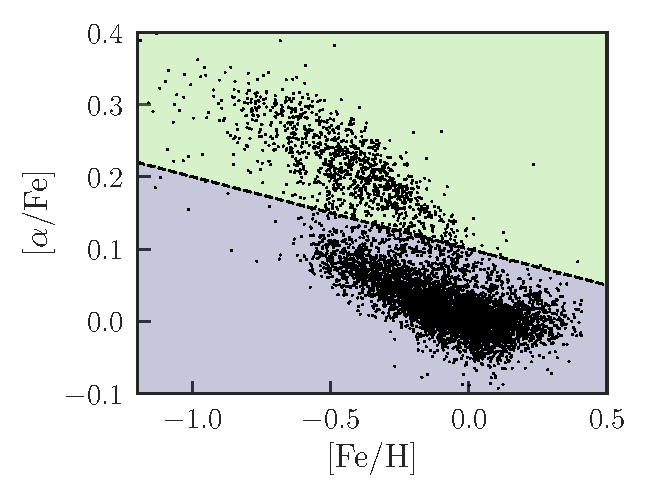
\includegraphics[width=0.8\textwidth]{thesis/Plots/afe_split_colors.pdf}
    \caption[The \feh{} and \afe{} abundances of stars in the solar vicinity from APOGEE DR14, indicating the bimodality in \afe{} at fixed \feh{}]{The \feh{}-\afe{} plane for stars located near the Sun (within 1 kpc) from the fourteenth data release (DR14 of the APOGEE survey). The coloured regions indicate a rough selection of stars with high (\emph{green}) and low (\emph{blue}) \afe{}. A bimodality in \afe{} is clearly present, at fixed \feh{}, between $-0.5 \lesssim \mathrm{[Fe/H]} \lesssim 0.0$ dex. The two populations appear to overlap at roughly solar \feh{}.}
    \label{fig:afe_split}
\end{figure}

These populations have, of course, been studied extensively since their discovery \citep[e.g.][]{1998A&A...338..161F,2003A&A...410..527B,2005A&A...433..185B,2013A&A...560A.109H,2014A&A...562A..71B,2014A&A...564A.115A,2014ApJ...796...38N,2015ApJ...808..132H} and, as expressed in Section \ref{sec:discsize}, have important links to the spatial structure of the Galaxy. Along with the MDFs (mentioned above), large scale spectroscopic surveys have also unveiled the stellar \feh{}-\afe{} distribution over great extents of the disc.  \citet{2014ApJ...796...38N} demonstrated that the positions of Red Clump (RC) stars in \feh{}-\afe{} space change as a function of Galactocentric cylindrical radius $R$ and height. Red Clump stars are helium burning, horizontal-branch stars whose luminosity is found to have very little dependence on both age and metallicty, and so make good standard candles. \citet{2015ApJ...808..132H} followed up on that work by showing a similar trend in a much larger sample of Red Giant Branch stars (albeit with less precise distance measurements). The findings of both studies were that the mean \feh{} of the low-\afe{} stars appears to move to higher \feh{} at smaller $R$, while the high-\afe{} stars dominate the distribution at high $z$, occupying a similar locus everywhere in the disc, but declining in density with $R$. These results place very strong constraints on any model which hopes to explain the origin of these element abundance trends, and I will briefly discuss such models in Section \ref{sec:galacticarchaeology}.

\subsection{The bulge and bar}

I discuss the bulge of the Milky Way in coordination with the bar, as these components are co-spatial in the center of our Galaxy and have a history and origin which is likely linked in some way, at some point in time. While the bulge is harder to study given the increased effect of extinction and problems with contamination by disc stars in bulge fields, a number of landmark studies have been able to elucidate its structure and its connection to the origin of the central region of the Galaxy.

\subsubsection{\emph{Pseudo}-bulges, boxes and peanuts}
During the early years of studying the Milky Way bulge, there was much debate as to its origin. The main arguments were either that it built up in the early history of the Galaxy through the merging of its satellite galaxy progenitors -- and thus is a `classical' bulge, resembling the structure of elliptical galaxies, which are thought to be built by the same process -- or that it formed in a secular fashion from stars in the disc or bar of the galaxy to become a `pseudobulge' \citep[a useful summary of these definitions is provided in Section 1.1 of][]{2004ARA&A..42..603K}. There now exists a wealth of evidence to suggest that while external galaxies certainly do host classical bulges \citep[e.g.][]{2009MNRAS.393.1531G}, the Milky Way itself is more likely host to a bulge with a structure indicative of secular processes - a pseudobulge. The Galactic bulge is boxy in shape \citep[e.g][]{1995ApJ...445..716D}, and is proposed to be formed via the heating of stars by buckling of a bar which formed from the stellar disc \citep[e.g.][]{1981A&A....96..164C,1991Natur.352..411R}.

As mentioned above, it was the work of \citet{1995ApJ...445..716D}, exploiting COBE infra-red data who revealed what is now referred to as the Boxy/Peanut (B/P) morphology of the Milky Way bulge. Prior to this, in perhaps the first direct evidence for a bar in the Milky Way, \citet{1991ApJ...379..631B} had shown the presence of asymmetry in $2.4 \mu$m balloon observations \citep{1982AIPC...83...48M} toward the Galactic centre, consistent with predictions for a bar of \citet{1979A&AS...37..403S} and \citet{1980ApJ...236..779L}. This broad picture of a B/P bulge plus a bar has prevailed to the present day, although the exact nuances of its structure are still the subject of debate.

Red Clump (RC) stars have proved to be essential in studying the structure of the Bulge.  Observing RC stars along lines of sight to the bulge allows for the mapping of its structure. Upon observing bulge RC stars Multiple groups find that there exists a split in the Red Clump at latitudes $|b| > 5^{\circ}$, where each branch of the split represents an RC population at a different distance, at either side of an X-shaped structure \citep{2010ApJ...721L..28N,2010ApJ...724.1491M,2011AJ....142...76S}. Later, using RC giants in the VVV survey, \citet{2013MNRAS.435.1874W} performed a more complete measurement of the 3D bulge structure, confirming the X-shape seen in the older observations. Recently, \citet{2016AJ....152...14N} used WISE images to make a clear imaging of the X-shape. Such X-shaped structures appear in many external disc galaxies \citep[e.g.][]{2006MNRAS.370..753B}, and are thought to arise as a consequence of the instabilities in the disc which give rise to the B/P morphology \citep[based on studies of N-body simulations, e.g.][]{2005MNRAS.358.1477A,2006ApJ...645..209D}.

Aside from morphological constraints on the bulge and bar, much effort has been made to model the dynamical effects of this structure on stars at the solar radius. As an example, it is contended by various groups that the Hercules stream in the solar neighbourhood (of stars moving together with heliocentric velocity $U \sim -30\ \mathrm{km\ s^{-1}}$ and $V \sim -50\ \mathrm{km\ s^{-1}}$), is the result of a perturbation by the outer Lindblad resonance (OLR) of a short ($\sim 3$ kpc), fast bar \citep{2000AJ....119..800D,2014A&A...563A..60A,2017MNRAS.466L.113M}. However, other groups claim that a longer bar ($\sim 5$ kpc) is necessary to best fit star counts from a variety of surveys \citep{2015MNRAS.450.4050W}, suggesting a more slowly rotating bar with an OLR further out in the disc \citep[although see][for a reconciliation of Hercules with a long, slow bar]{2018MNRAS.477.3945H}. The connection between the bar and the local velocity distribution, and the current model of the disc origin for the Milky Way bulge are both suggestive of the importance of understanding the complexities of the interaction between the different components of the Galaxy.

\subsubsection{Element Abundances and the Age of the Bulge}
Where element abundances are considered, the central regions of the Galaxy bear some similarities to the disc, and some important differences. Early studies of abundances in the bulge relied on small samples in regions of low extinction \citep[e.g.][]{1994ApJS...91..749M}, revealing that stars in these regions had an intermediate metallicity (\feh{} $\sim -0.25$ dex), and were enhanced in Aluminium. The vertical gradient of \feh{} across the bulge is negative, which was originally considered incompatible with a purely disc origin of this component, and suggesting that the Milky Way had at least some classical bulge component \citep[e.g.][]{2008A&A...486..177Z}, however the kinematics of the bulge place very low upper limits on the mass of this component \citep[e.g. $\sim 8\%$;][]{2010ApJ...720L..72S}. A closer look at the metallicity distribution in the bulge with better data from the ARGOS survey revealed that the bulge stars divide into sub-populations in \feh{} space, amounting to a wide MDF spanning a range $-2.8 \lesssim \mathrm{[Fe/H]}\lesssim 0.6$ dex \citep{2013MNRAS.430..836N}. The ARGOS data appear to be consistent with an entirely disc-instability driven origin of the bulge.

Alternate element abundances which provide a way to test models for the bulge formation are $\alpha$-elements, which trace star formation as described in Section \ref{sec:discabundances}. Many bulge stars have enhanced \afe{}, and appear similar in their \afe{} and \feh{} to local stars in the \afe{} enhanced disc \citep{2010A&A...513A..35A,2015A&A...584A..46G}, suggesting a similar timescale for star formation. However, by taking high resolution spectra of microlensed dwarfs in the bulge, \citet{2013A&A...549A.147B} found that the `knee' in the bulge \afe{}-\feh{} plane (which is present at the solar radius in the high-\afe{} population of Figure \ref{fig:afe_split}) is at a slightly higher \feh{} than in the local disc, suggesting a slightly faster enrichment history in the center of the galaxy. The \afe{}-\feh{} distribution as seen by APOGEE in different radius and height bins from the Galactic center to the solar vicinity \citep{2016PASA...33...22N} also seems to suggest that the high-\afe{} stars in the solar vicinity are in some way connected to those in the central region of the Galaxy.

In terms of stellar age, the bulge is generally considered to be built of relatively old stars, at least older than those in the disc. The mean age of the bulge which can be measured from the colour-magnitude diagrams of giant stars in the bulge obtained from deep photometry is $\sim 10$ Gyr \citep[e.g.][]{2003A&A...399..931Z,2013A&A...559A..98V}, and it seems that there are very few stars younger than $\sim 5$ Gyr \citep{2011ApJ...735...37C}. Measuring ages using colour-magnitude diagrams in the bulge is notoriously difficult owing to difficulties in subtracting foreground disc contaminants, and uncertainties in reddening estimates and (usually) unmodelled effects of the metallicity distribution, leading to uncertainties of the order of $\sim 2$ Gyr \citep{2016ASSL..418..199G}. A very old bulge is interpreted as being indicative of one built via merging processes (a classical bulge), given that disc instabilities should bring young stars into the bulge. The microlensed dwarf sample of \citet{2013A&A...549A.147B} suggests that there may indeed be a population of young stars in the bulge, finding that 22\% of the dwarfs were younger than 5 Gyr old. Therefore, it seems that finding accurate age estimation methods for giants in the bulge may be able to provide stronger constraints on the classical vs. pseudobulge problem.

\subsection{The stellar halo}
The halo of the Milky Way is the component which is least affected by dust extinction (at least above and below the plane of the disc). The halo can undoubtedly provide a wealth of information on the history of the Galaxy, owing to the fact that dynamical timescales are much longer than in the disc or bulge, preserving dynamical traces of past merger events in the form of coherent stellar debris referred to as streams \citep[e.g.][]{1996ApJ...465..278J}. The halo and the stellar substructure within it may be among the best means of measuring the mass and inferring the gravitational potential of the Milky Way halo \citep[e.g.][]{2014ApJ...794....4P}. For this reason, the detailed understanding of its structure and the origin of it is of great importance to developing a complete picture of the formation of the Galaxy. Here I will briefly touch upon some of the important features of the halo and how these connect to its overall evolution.

\subsubsection{Structure}
As mentioned above, the long dynamical timescale in the halo means that phase space substructures are likely not readily erased. A good example of such a structure is the Sagittarius dwarf galaxy, which has survived at least one or two orbits around the Galaxy \citep[e.g.]{1999AJ....118.1719J}, if not many more \citep[e.g.][]{1997AJ....113..634I}, as evidenced by its stellar stream which wraps entirely around the galaxy and is mapped over $\sim 100$s of degrees \citep[e.g.][]{2003ApJ...596L.191N,2004AJ....128..245M,2006ApJ...642L.137B,2009ApJ...700.1282Y}. Sagittarius is just one of a panoply of known groups of accreted stellar material \citep[see e.g.][for a review]{2013NewAR..57..100B}, which indicate that at least some part of the stellar halo is built from the accretion of smaller systems \citep[as predicted in the seminal work of][which I discuss further in Section \ref{sec:galacticarchaeology}]{1978ApJ...225..357S}. These lumps in the density profile of the halo must be accounted for when measuring its overall structure \citep[e.g.][]{2011MNRAS.416.2903D}. The mass in stellar substructure in the halo must also be accounted for when estimating its total stellar mass, and is estimated to be of the order of $10^8\ \mathrm{M_{\odot}}$ \citep[based on a recent review by][]{2016ARA&A..54..529B}. Once substructure is accounted for, then the stellar halo can be fit with a relatively smooth density model. Including the mass in this smooth component, the total stellar mass of the halo is estimated to be in the range of $4-7\times 10^{8}\ \mathrm{M_{\odot}}$ \citep{2016ARA&A..54..529B}.

The density distribution of the smooth part of the halo is well characterised using a variety of tracers whose distances can be determined to a good level of accuracy, such as RR Lyrae stars 
\citep[e.g.][]{2009MNRAS.398.1757W,2010ApJ...708..717S,2013AJ....146...21S,2014ApJ...788..105F}, blue horizontal branch (BHB) and blue straggler stars \citep[e.g.][]{2011MNRAS.416.2903D}, main-sequence turn-off (MSTO) stars \citep[e.g.][]{2011ApJ...731....4S} and red giant branch (RGB) stars \citep[e.g.][]{2015ApJ...809..144X}; a good overview of the results from all of these studies can be found in \citet{2016ARA&A..54..529B}. The halo density profile is fit across all these studies by power-law, with an index $\sim-2.5$ in the inner parts. Additionally, most of the aforementioned works agree that the inner halo is flattened somewhat, by a factor of $\sim 0.65$. It is also generally agreed, from the farthest reaching data, that the density profile steepens with radius with a break in the power-law at a break radius $r_{\mathrm{b}}\sim 20$ to $25$ kpc \citep[e.g.][]{2009MNRAS.398.1757W,2011ApJ...731....4S,2011MNRAS.416.2903D}. Such a break in the halo density profile is thought to be related to the accumulation of stars at the apocenter of a relatively massive accretion event(s) which is now well mixed into the smooth halo \citep{2013ApJ...763..113D}, and is not a ubiquitous feature of galaxy haloes \citep[a good example being the lack of such a break in M31, e.g.][]{2011ApJ...739...20C}. Therefore, while the structure of the Milky Way halo may be common in some sense, with substructure and smooth stellar light similar to that seen in external galaxies, it may also have some significant structural differences, such as its broken profile. 

\subsubsection{\emph{In situ} and \emph{ex situ}}
While the overall density profile of the halo is generally agreed upon, there is significant debate over the origin of its stellar populations, particularly regarding the fraction of stars which were formed within the Galaxy (i.e. \emph{in situ}), and those which were brought in after forming inside satellite galaxies (\emph{ex situ}). Perhaps the most contentious of these debates began with the findings of \citet{2007Natur.450.1020C}, and the later work of \citet{2012ApJ...746...34B}, who proposed that the halo consists of inner and outer structural components, the inner having prograde rotation and the outer retrograde, indicating that they likely formed differently. Such \emph{in situ} components are a common feature of galaxies in cosmological simulations \citep[e.g.][]{2011MNRAS.416.2802F,2012MNRAS.420.2245M}, where in some cases, disc stars are heated vertically to become part of the inner halo \citep[there appears to be evidence for such stars in M31, e.g.][]{2013ApJ...779..103D}. However the existence of a clear dual halo in the Milky Way was strongly contested by the work of \citet{2014ApJ...786....7S}, who contended that the kinematics were well fit by a single halo which had significant substructure. Ejection of disc stars into the halo to form some \emph{in situ} component is perhaps not so outlandish, given the recent connection of the Triangulum-Andromeda overdensity (a group of stars lying far above the plane of the Galaxy, $z \sim 10$ kpc) with the disc \citep{2015MNRAS.452..676P,2018Natur.555..334B}.

\subsection{Summary}
Having given an overview of the structure of the Milky Way as it is known today, it is clear that it presents a number of characteristics which already suggest that it may not be a typical example of a disc galaxy. I have also discussed how the Milky Way is host to some features that are ubiquitious among disc galaxies, which will be useful in extrapolating galaxy formation models beyond our Galaxy. In summary, the important aspects of the Galactic structure identified here are as follows:
\begin{itemize}
    \item The disc of the Galaxy is host to a complex spiral structure, with a possible maximum of four arms as traced by the youngest stars \citep[e.g.][]{2014MNRAS.437.1791U} - although old stars trace out only two arms \citep[e.g.][]{2000A&A...358L..13D}. This may be indicative that the spiral structure arises in a transient fashion \citep[e.g.][]{2011MNRAS.410.1637S}, rather than being stationary waves within the disc \citep[e.g.][]{1964ApJ...140..646L}. In this sense the Milky Way appears to be roughly consistent with being a typical Sb/c galaxy, in terms of morphology.
    \item The disc appears to have a shorter scale length than other disc galaxies at a similar mass \citep[e.g.][]{2010MNRAS.406.1595F} by a factor of $\sim 2$.
    \item The ratio of $\alpha$ element abundance to that of Iron, \afe{} has a characteristic bimodality at fixed \feh{} at the solar radius, with each population having a seemingly distinct structure in terms of scale length but mixing in vertical height \citep[e.g.][]{2012ApJ...751..131B,2012ApJ...753..148B,2016ApJ...823...30B}. High-\afe{} stars are also found in the bulge of the Galaxy, and indicate a rapid and intense early star formation history \citep[e.g.][]{2017arXiv170202971B}.
    \item The bulge appears to be mainly of a disc origin, with stars removed from the disc via buckling instabilities in the Galactic center, giving rise to a distinctive `Box-Peanut' morphology \citep[e.g.][]{2005MNRAS.358.1477A}.
    \item The Galaxy certainly has a bar at its center, but its length and pattern speed are presently a subject of debate \citep[e.g.][]{2000AJ....119..800D,2015MNRAS.450.4050W}. Understanding the origin of the bar and its connection to the X-shaped structure seen toward the Galactic bulge \citep[e.g.][]{2016AJ....152...14N} and in the bulges of external galaxies \citep{2006MNRAS.370..753B}, is an essential constraint on the cosmological context of the Milky Way.
    \item The halo of the Milky Way contains an abundance of substructure \citep{2013NewAR..57..100B}, which can be used to directly study the assembly of the Galaxy in detail.
    \item The smooth component of the halo is well measured \citep[e.g.][]{2011MNRAS.416.2903D}, and has a characteristic break at $r\sim 25$ kpc, which is not ubiquitous among other galaxy stellar haloes \citep[e.g.][]{2013ApJ...763..113D}. The origin of the stellar populations which make up the smooth halo are contentious at present \citep[e.g.][]{2007Natur.450.1020C,2012ApJ...746...34B,2014ApJ...786....7S}.
\end{itemize}

While these examples of characteristic properties of the Milky Way provide some insight into its origin and place as a disc galaxy, they only scratch the surface of an abundance of work and efforts to properly characterise our Galaxy. However, the overview I present here is intended to merely provide some context to the work I present in this thesis. These constraints and others are crucial elements in formulating robust models for the formation of the Milky Way, some aspects of which I will discuss in the following sections.
%\subsection{The Local Group}

\section{Unearthing fossilised galaxy formation in the Milky Way}
\label{sec:galacticarchaeology}

I have thus far presented an overview of our current knowledge of the Milky Way at the present day, touching upon its wider context as a disc galaxy. The aim of this section is to introduce and review the current understanding of how the Galaxy came to have these features, with a particular focus on the disc and the solar neighbourhood, which are the main concern of this thesis. The use of the present day features of the Galaxy as constraints on models for its formation is commonly referred to as `Galactic archaeology'; the different components of the Galaxy are treated as fossils with which we can understand the history of the Galaxy (in this analogy, the term `Galactic palaeontology' is perhaps more appropriate). The following chapter acts as a review of this practice, with a view to presenting the state of the art upon which I hope to build in this thesis.

\subsection{Galaxy disc formation to first order}

% A useful way to further review the wealth of work on the formation of the Milky Way is to describe a schematic of its formation as a disc galaxy, as unveiled by studies of it throughout the last century. The conception of the `canonical' model for the birth of the Milky Way in a rapid collapse of a proto-galactic gas cloud \citep[the ELS model;][]{1962ApJ...136..748E} makes a good starting point for such a schematic. 

In what can be considered as the first implementation of Galactic archaeology, \citet[the ELS model]{1962ApJ...136..748E} showed that the orbital energies and eccentricities of stars with lower metallicities were higher than those of their metal-rich counterparts, inferring that the former were members of the first generation of stars formed from the originally rapidly collapsed protocloud of the Galaxy. The later work of \citet[the S\&Z model]{1978ApJ...225..357S} inferred that the age, metallicity and spatial distribution of Galactic globular clusters (GCs) suggested a different view of the formation of the Galaxy through the coalescence of `proto-galactic fragments'. These seminal works underpin many of the modern studies of the Milky Way, and are commonly framed as competing scenarios. However, at the time, these findings mirrored the developments in the CDM model \citep{1978MNRAS.183..341W}. Analytical models of the collapse of gas in a halo which gained angular momentum from hierarchical clustering -- a kind of ELS-S\&Z hybrid -- produced seemingly realistic discs \citep{1980MNRAS.193..189F}, with density distributions described by exponential laws. Such exponential density laws are to be expected given observations of external galaxy discs \citep[e.g.][]{1959HDP....53..311D,1970ApJ...160..811F,1983MNRAS.202.1025G,2006A&A...454..759P}. Since these early analytic models, it is now realised that such a collapse would likely produce unrealistically small discs \citep[e.g.][]{2000MNRAS.317..697E}. More recently, the redistribution or 'scrambling' of the angular momentum of individual stars has been invoked as an alternative and more likely means of producing exponential disc profiles \citep[e.g.][]{2013ApJ...775L..35E,2016ApJ...830..115E,2016arXiv161203171H}. While analytic approaches and idealised N-body simulations would work well at describing isolated galaxy disc formation, hydrodynamical simulations in a cosmological context struggled to produce realistic populations of disc galaxies until advances in the inclusion of detailed feedback models, as discussed in Section \ref{sec:galaxyhaloconnect}. 

The importance of feedback processes in shaping disc galaxies both structurally and in terms of element abundances cannot be overstated. Early cosmological simulations had significant issues with angular momentum loss following mergers, and produced galaxies with unrealistically large bulge components \citep[this became known as the `angular momentum catastrophe' e.g.][]{1994MNRAS.267..401N}. However, significant improvements in the ability of simulations to model and resolve feedback processes lead to a step-change in the ability of cosmological simulations to predict the formation of realistically sized disc galaxies \citep[e.g.][among many others]{2011ApJ...742...76G,2012MNRAS.426..690B,2012MNRAS.427..379M,2013MNRAS.436..625S,2014MNRAS.445..581H,2014MNRAS.442.2474M,2014MNRAS.443.2452M}, with the key factor being the ability of the feedback models to drive realistic outflows in the simulated galaxies \citep[e.g.][]{2008MNRAS.387.1431D,2008MNRAS.389.1137S}. Such outflows pause star formation in the galaxies and eject gas into the halo, giving time for the discs to gain angular momentum, before the gas is re-accreted at later times, forming realistic, extended discs. These subgrid models parameterise the effects of feedback in an \emph{ad hoc} fashion, owing to the fact that the detailed dynamical processes from which they arise are generally unresolved. However, through calibration of these models to reproduce large scale aspects of the galaxy population, such as the galaxy stellar mass function, stong predictive power can still be achieved \citep[good discussions of this are given in][]{2015MNRAS.446..521S,2015MNRAS.450.1937C}. The fact that these patterns of inflow and outflow are required to model realistic discs in a cosmological context suggests very strongly that these are a significant aspect of the physics that shaped the Milky Way and other disc galaxies.

From the preceding discussion then, it is clear that, to first order, we can picture the Milky Way disc as initially formed by some collapse of primordial gas \citep[as in][]{1962ApJ...136..748E}, which gained angular momentum from merging satellites \citep[e.g.][]{1978ApJ...225..357S} and became flattened into a disc, compressing the gas and triggering star formation. This star formation results in stellar feedback, driving gas from the disc, slowing the star formation and gas collapse and preventing the formation of a massive spheroidal component. The outflowing gas can then be re-accreted at late times, extending the disc. It is also clear, given the predictions of the CDM model, and the existence of stellar substructure in the haloes of the Milky Way and other disc galaxies, that the Galaxy likely also underwent much merging and accretion of \emph{ex-situ} material during this evolution, all of which shape the Galaxy that we observe today. In the following sections I will review the recent findings of Galactic archaeology, and use these to assess and refine this simple picture, and identify gaps in our understanding of the evolution of the Milky Way.

\subsection{Confronting models with data}

Galactic palaeontologists have a number of tools at their disposal, with which the history of the Milky Way can be unearthed. While observational tracers such as stellar populations and their element abundances, ages, spatial distributions and kinematics are a crucial element in placing constraints on models of the formation and evolution of the Milky Way, such as those reviewed in Section \ref{sec:mwadg}, the models themselves and the techniques used to make them are perhaps just as important a tool. The strongest conclusions about the formation of the Galaxy can only be attained when models are confronted with data, and so combining observation and theory is a key aspect of Galactic palaeontology.

A useful example of this, and one which I will return to at length in the course of this thesis, is the prediction of the origin of the bimodality in \afe{} at the solar radius, for which I discussed the observational constraints in Section \ref{sec:discabundances}. Since these disc populations with markedly different \afe{} at fixed \feh{} very likely result from different star formation histories, it is challenging to reconcile their co-spatiality in the Galactic disc with the predictions of one-zone chemical evolution models \citep[e.g.,][]{1959ApJ...129..243S,1963ApJ...137..758S}. While such simple models essentially inaugurated the field of quantitative chemical evolution modeling, they had important limitations.  The most important of which was their failure to reproduce the metallicity distribution function (MDF) of stars in the solar neighbourhood \citep[known as the `G-dwarf problem',][]{1962AJ.....67..486V,1963ApJ...137..758S}. This motivated the development of more detailed chemical evolution models, for example, allowing for the consideration of gas inflow \citep{1972Natur.236...21L,1977ApJ...216..548T}, radial gas flow \citep[e.g.][]{2000A&A...355..929P}, and eventually the decomposition of the Galactic disc into concentric evolution zones to capture the effects of `inside out' formation \citep[e.g.][]{1976MNRAS.176...31L,1980FCPh....5..287T,1989MNRAS.239..885M}. 

Over the past two decades, two classes of analytic models in particular have attracted attention, owing to their ability to reproduce broadly the observed elemental abundance trends in the solar neighbourhood, and abundance gradients throughout the disc. These are i) models in which the high- and low-\afe{} components of the discs form in response to distinct episodes of gas accretion, during which gas is consumed at different rates \citep{1997ApJ...477..765C,2001ApJ...554.1044C,2009IAUS..254..191C}; and ii) models in which the two components represent the equilibrium star formation conditions in different parts of the disc, but later become co-incident as a consequence of the radial mixing of stars \citep{2009MNRAS.396..203S,2009MNRAS.399.1145S}. 

The `two-infall model' of \citet{1997ApJ...477..765C,2001ApJ...554.1044C}, invokes an intense initial phase of star formation whose brevity precludes enrichment of the interstellar medium (ISM) by Type Ia SNe, thus resulting in the formation of the high-\afe{} sequence. A hiatus in star formation is then invoked, during which the unconsumed fraction of the gas delivered by the first infall (which is assumed to remain in place without consumption by star formation or ejection by feedback) is enriched by Type Ia SNe, reducing its \afe{}. A second, more prolonged episode of gas infall then triggers the steady formation of the stars comprising the low-\afe{} sequence. The `radial migration' model of \citet{2009MNRAS.396..203S} assumes a continuous, smoothly-varying delivery of gas to the disc, but allows for the exchange of star-forming gas and stars between adjacent radial bins. This allows for the present-day co-location of disc stars whose formation conditions (and hence their location in \afe{}-\feh{} space) differed significantly. Bimodality of \afe{} at fixed \feh{} therefore stems, in this model, from such a superposition of populations, fostered by the outward migration of high-\afe{} stars that formed rapidly close to the Galactic centre, and the (lesser) inward migration of low-\afe{} stars formed farther out in the Galactic disc. 

 In an effort to scrutinise the viability of these scenarios and assess their sensitivity to the variation of free parameters, \citet{2016arXiv160408613A} used their flexible analytic chemical evolution model \textsc{flexCE} to implement the models in a consistent framework. They concluded that both models are able to produce high- and low-\afe{} sequences, but identified potential shortcomings in both: the two-infall model required fine-tuning of the duration of the star formation hiatus and was incapable of yielding the bimodality in \afe{} over an extended a range of \feh{} seen by APOGEE \citep[seen in, e.g.][]{2014ApJ...796...38N,2015ApJ...808..132H}. Additionally their implementation of the radial migration scenario produced a weaker bimodality than that revealed by APOGEE, where the `valley' between the populations is filled. These failings of analytic models highlight the need for more flexible means of understanding Galactic chemical evolution.
 
 Models such as those described above are useful, but do require a great deal of fine tuning to reproduce the data \citep[complex models can have greater than 10 free parameters][]{2016arXiv160408613A}. With the introduction of higher resolution data with a wider coverage of the Galaxy, these analytic approaches require greater levels of such tuning, eventually becoming very complex, and likely unrealistic as a result. A potentially more fruitful method of developing robust models and making strong predictions for the evolution of the Milky Way, without recourse to such complexity, is through ab initio numerical simulations. Simulations take on a variety of forms. The simplest simulations model a single Milky Way-like galaxy using only gravitationally interacting particles (i.e. N-body only simulations),  whereas the most detailed simulations self-consistently model the interaction of gas, stars and dark matter, including prescriptions for star formation, feedback and -- in the most state of the art models -- the effects of magnetic fields and the modelling of radiative transfer.
 
 Among the many methods and types of simulations of Milky Way-like galaxies, the most widely applied to Galactic archaeology are cosmological `zoom-in' simulations, which extract Milky Way-like haloes from lower resolution, large volume cosmological simulations, and re-simulate them at very high resolution, usually including baryonic effects and modelling their star formation and chemical evolution histories. Early applications of the zoom-in technique studied the formation of early type galaxies \citep[e.g.][]{1993ApJ...412..455K}, owing to the fact that early implementations of it lended themselves to more massive galaxies, with early accretion histories. Developments in the technique \citep[such as those described in][alongside those in the sub-grid models, as described earlier]{2009ApJ...707..250M} lead to the simulation of more realistic Milky Way analogues \citep[e.g.][]{2012ApJ...756...26M}, which eventually allowed for new predictions for the contribution of merging and radial migration to the element abundances at the solar radius \citep[e.g.][]{2013A&A...558A...9M,2014A&A...572A..92M}. Other similar simulations produced structural components resembling the thin and thick disc, and reproduced the element abundances in the Milky Way with some success \citep{2012MNRAS.426..690B}. 
 
 Such simulations have had a great deal of success in producing structurally realistic Milky Way analogues, and have revealed a number of competing scenarios for the formation of vertically extended stellar components. In brief, these can be summed up as: a) the heating of an initially thin disc by relatively massive mergers \citep[e.g.][]{2008MNRAS.391.1806V,2009ApJ...700.1896K}, b) the formation of successively thin stellar populations out of a compressing gas disc \citep[e.g.][]{2013ApJ...773...43B,2017arXiv170901040N} or one which is heated by gas rich mergers at early times \citep[e.g.][]{2004ApJ...612..894B,2013A&A...558A...9M}, and c) the direct accretion of stars onto vertically extended but disc-like orbits \citep[e.g.][]{2003ApJ...597...21A}. All of these scenarios can somewhat explain the spatial structure of the disc, but most struggle to adequately explain the element abundances at the solar radius. Indeed, some simulations do not track the evolution of chemical abundances self-consistently, with many resorting to `painting' abundances onto particles in post-processing. For this reason, it may be more straight-forward to compare stellar ages in the simulations with their observational counterparts - although, as will be touched upon in Chapter \ref{chapter:apogeestruc}, robust age measurements for large stellar samples are inherently difficult to obtain.
 
\section{Summary and thesis outline}

This thesis has consisted thus far of an overview of the field of Galactic archaeology, discussing the Galaxy and disc galaxies from the `top-down', examining work on galaxy formation in a cosmological context, then describing some of the current understanding of the structure of the Milky Way itself and finally introducing Galactic archaeology and some of the currently proposed models for the formation of the Galaxy. Returning to the overarching question of the typicality of the Milky Way which underlies this thesis, I have also discussed how the current literature provides constraints on this question. 

In the following chapters, I intend to perform Galactic archaeology using the most up to date data available for the Milky Way, and studying the current state-of-the-art in large volume hydrodynamical simulations of galaxy formation in a cosmological context. In detail:
\begin{itemize}
    \item In Chapter \ref{chapter:apogeestruc}, I measure the spatial density structure of the Milky Way stellar disc as a function of age and metallicity. The goal of this chapter is to establish what the present day structure of the disc is, and to try and place constraints on its evolution chronologically. Providing a robust map of the disc structure in mono-age populations provides robust constraints on models for the evolution of that structure over cosmic time.
    \item Chapter \ref{chapter:eagle} presents an examination of the element abundances of discs of Milky Way mass galaxies in the EAGLE simulations. In it, I present a new model for the origin of $\alpha$-element bimodality at fixed \feh{} in the Milky Way, based on the origin of this feature in galaxies within the simulation. The simulations make predictions for the low and high-\afe{} disc populations in the Milky Way and provide insights into the typicality of the Galaxy on the basis of this feature.
    \item In Chapter \ref{chapter:highe}, I present the serendipidous discovery of a large population of accreted stars in the stellar halo of the Milky Way, which can be associated to the merging onto the Milky Way of a relatively massive dwarf galaxy. I assess the origin of satellite debris in the EAGLE simulations, which allows me to place constraints on the stellar mass of the accreted Milky Way system, and also to understand the commonality of accretion events such as this onto Milky Way mass galaxies.
\end{itemize}
Following these main chapters, I will present the general conclusions of the thesis, before outlining the future of the field, and the further work which will be necessary to better constrain the formation, evolution and typicality of the Galaxy.




